\documentclass[border=5pt]{standalone}
\usepackage{tikz}
\usetikzlibrary{calc}
\usepackage{amsmath}
\begin{document}
    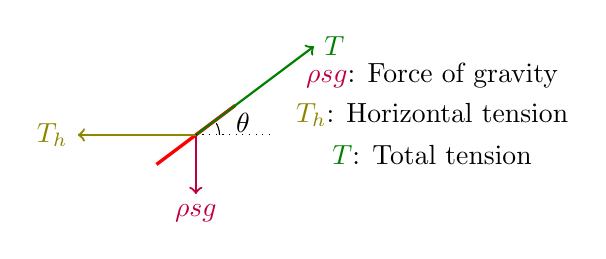
\begin{tikzpicture}[scale=1]
        % Draw a small segment of the chain
        \draw[very thick, red] (0.5,0.375) -- (1.5,1.125);

        % Draw force vectors
        \draw[->, thick, purple] (1,0.75) -- (1,0) node[below] {$\rho sg$};
        \draw[->, thick, olive] (1,0.75) -- (-0.5,0.75) node[left] {$T_h$};
        \draw[->, thick, green!50!black] (1,0.75) -- (2.5,1.875) node[right] {$T$};



        % Draw angle θ
        \draw[black] (1.3,0.75) arc (0:30:0.3);
        \node at (1.6,0.9) {$\theta$};
        \draw[dotted] (1,0.75) -- (2,0.75);


        % Add legend
        \node[align=left] at (4,1.5) {
            \textcolor{purple}{$\rho sg$}: Force of gravity};
        \node[align=left] at (4,1) {
            \textcolor{olive}{$T_h$}: Horizontal tension};

        \node[align=left] at (4,0.5) {
            \textcolor{green!50!black}{$T$}: Total tension};
    \end{tikzpicture}
\end{document}
